\chapter{MVVM 模式与 Reactive Programming}

前三章介绍了项目的背景、需求以及基本的概要设计,本章将着重介绍围绕 MVVM 模式进行的分析与设计活动。

本章将用一定的篇幅详细介绍 MVVM 模式在面向对象的命令式编程语言内的设计实现。使用实例解释 Reactive Programming 以及 FRP 的特性,并导出基于 Reactive Programming 模式的 ViewModel 实现方案。

\section{用户交互与异步编程模型}

用户与计算机的交互是基于人机交互界面(UI)进行的,早期的终端用户界面 (Console User Interface, CUI) 程序与用户进行同步交互,交互的模型为: 用户输入-程序执行-程序输出-用户输入\ldots,这样的逻辑在面向过程编程的语言实现中是非常自然的程序表达——按先后顺序执行每一条语句。

在图形界面(Graphical User Interface, GUI)得到应用之后,用户可以不间断地与程序进行交互而不需要等待程序的执行,这样的设计极大的提升了用户体验。现代的 GUI 程序广泛使用了事件模型处理用户交互,事件是一组时间顺序的离散数据的集合,对程序来说事件是一类异步产生的数据,因此,基于事件进行编程便成为了进行用户交互实现的基本方法。

明确了这点之后,我们可以将行用户交互实现的本质问题归结为~\textbf{处理异步事件}。

基于事件的开发并不是命令式(Imperative)编程模式所擅长的领域,也导致了大多数 GUI 程序的交互实现都极其不易维护。

以 Drag'n'Drop (拖放操作, DnD) 为例\cite{Zhao2010},在 GUI 上实现 DnD 操作需要程序监听三个不同的 GUI 事件:

\begin{itemize}
  \item 在 MouseDown 事件中标记 isDragging (正在拖动)
  \item 在 MouseMove 事件中判断 isDragging 并且开始绘制拖放光标、使用 API 获取拖放的数据
  \item 在 MouseUp 事件中判断 isDragging 并结束拖放状态(停止绘图)
\end{itemize}

在命令式编程语言中往往使用回调函数(Callback Function)对事件进行处理,这种离散的逻辑碎片导致了在 GUI 实现中出现大量的碎片代码以及全局状态,破坏了“代码逻辑局部性”、“变量局部性”等有利于代码组织和维护的性质。

下面几个小节将就异步编程模型问题对 MVC 与 MVVM 框架进行讨论。

\section{MVC 架构模式}

MVC 架构模式中系统被分成 Model(模型)、View(视图)、Controller(控制器) 三个部分

\begin{figure}[!h]
  \begin{center}
    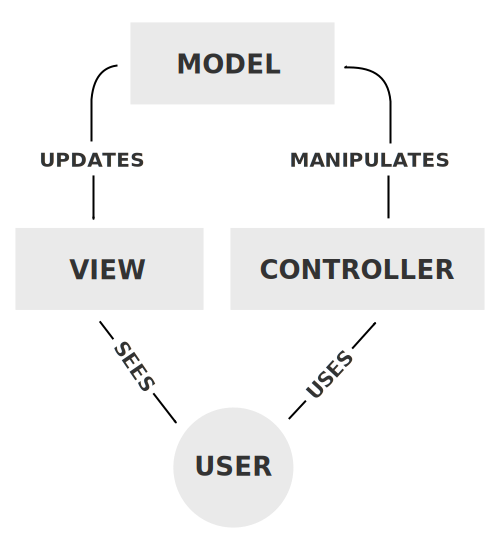
\includegraphics[scale=0.5]{figures/MVC-Process.pdf}
    \caption{MVC 模式}
  \end{center}
\end{figure}

\begin{itemize}
  \item \textbf{Model} 用于处理数据和业务操作
  \item \textbf{View} 负责控制 Model 的显示逻辑
  \item \textbf{Controller} 响应用户事件、更新 Model
\end{itemize}

直接应用 MVC 模式处理异步逻辑~\footnote{实现上文的 Drag'n'Drop 例子} 非常容易出现下面这样的 Controller 逻辑:

\begin{verbatim}

    boolean isDragging;

    view.on('mousedown', () => {
      isDragging = true
      setPointerIcon()
    })

    view.on('mouseup', () => {
      isDragging = false
      setPointerIcon()
      handleDnD()
    })

    view.on('mousemove', () => {
      if (isDragging) {
        drawEffect()
      } else {
        doSomething()
      }
    })

\end{verbatim}

上面的代码依赖“全局状态”并且同一个逻辑被分散到了几个代码块中,可以看到这样的实现是比较缺乏可维护性和可读性的。

当然,上面的实现只是 Controller 对异步逻辑的实现中最糟糕的例子。MVC 设计模式并没有对这一部分的逻辑进行更加详细的设计,因此,在 MVC 设计模式的基础上 Microsoft 提出了基于观察者模式(Observer Pattern)的 Controller 实现,也就是下文将讨论的 MVVM 模式。

\section{面向对象的 MVVM 实现}

MVVM 模式是对 MVC 模式的一种特殊形式,本节将就 MVVM 模式以及其应用的 Observer 设计模式进行讨论。

\begin{figure}[!h]
  \begin{center}
    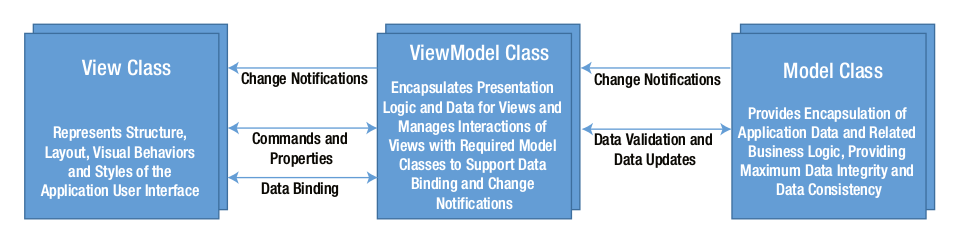
\includegraphics[scale=0.5]{figures/diagram-mvvm-pattern-ref.png}
    \caption{MVVM 设计模式中的关键类~\cite{ghoda2012windows}\label{MVVMCoreClasses}}
  \end{center}
\end{figure}

ViewModel 在 View 与 Model 中间进行数据处理、转换,是 MVVM 模式中的重要角色。

简要描述一下 MVVM 结构中的基本交互: ViewModel 通过监听 Model 变更对 View 进行更新; View 通过 ViewModel 将用户事件转换为 Model 数据、对 Model 进行更改。

Model 与 ViewModel、View 与 ViewModel 之间的通信由 Binder 机制实现。Binder 机制是 MVVM 的 WPF 实现内隐含的设计~\footnote{MVVM 的命名并没有表现 Binder 机制},通过 Binder 实现 ViewModel 到 View 的属性绑定和 ViewModel 对 Model 的监听。

在概述中我们也提到 MVVM 架构设计的一个亮点在于 ViewModel 在行为上与 Model 保持的一致性,因此 ViewModel 之间的通信也是通过 Binder 进行的。

在面向对象的设计模式中容易发现观察者模式(Observer Pattern)是非常适合这种场景的。因此,WPF 中使用的 ViewModel + Binder 借口就派生于观察者模式。

\begin{figure}[!h]
  \begin{center}
    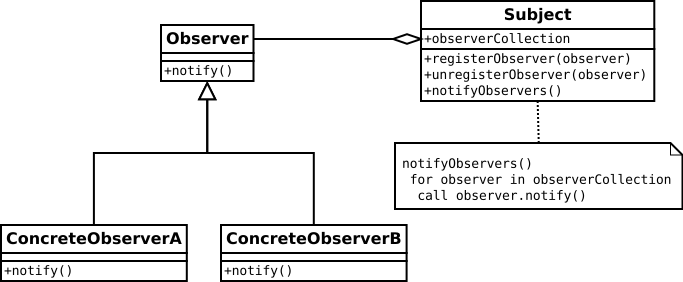
\includegraphics[scale=0.6]{figures/pattern-observer.pdf}
    \caption{观察者模式\label{PatternObserver}}
    Subject 接受注册 Observer 并在 notifyObserver 中向 Observer 推送数据
  \end{center}
\end{figure}

参照图~\ref{PatternObserver}~\footnote{Wikipedia: File:Observer.svg} 中的定义对 Model 与 ViewModel 进行定义:

\begin{verbatim}
    @interface IModel implements ISubject;
    @interface IViewModel implements IObserver;
\end{verbatim}

为了让 ViewModel 具有与 Model 相似的行为,将 ViewModel 的接口改写为:

\begin{verbatim}
    @interface IViewModel implements IObserver, IModel;
\end{verbatim}

\begin{figure}[!h]
  \begin{center}
    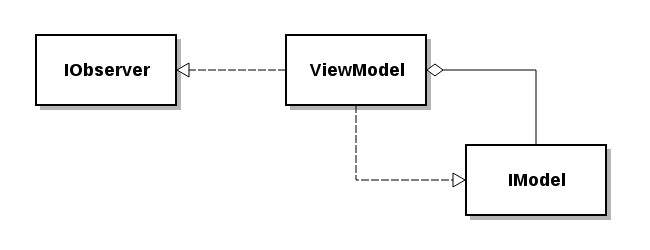
\includegraphics[scale=0.5]{figures/diagram-viewmodel.png}
    \caption{ViewModel 类图\label{ViewModelClass}}
  \end{center}
\end{figure}

ViewModel 通过订阅 Model 获取 Model 的数据变更(图~\ref{MVVMCoreClasses} 中 Model 至 ViewModel 的 $Change Notifications$)。与之类似,View 与 ViewModel 之间的 Binder 定义:

\begin{verbatim}
    @interface IBinder implements ISubject, IObserver;
\end{verbatim}

Binder 实例构造时指定 View 元素作为 Observer 实例,指定 ViewModel 元素作为 Subject 实例就可以建立 ViewModel 至 View 的单向绑定关系。双向绑定关系由两个单项绑定构成,不加赘述。

值得一提的是,由于 ViewModel 同时实现了 Model 接口,具备了 Model 的行为特性,ViewModel 之间也是可以互相观察的:

\begin{figure}[!h]
  \begin{center}
    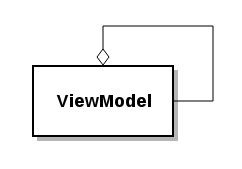
\includegraphics[scale=0.5]{figures/diagram-viewmodel-cascading.png}
    \caption{ViewModel 可级联的特性\label{ViewModelCascading}}
  \end{center}
\end{figure}

这样的设计使得ViewModel模式获得了很强的可扩展性,将用户交互状态分开给不同的 ViewModel 进行管理可以显著减小业务逻辑状态的维护难度,开发者可以利用封装的 ViewModel 类库进行组合来完成用户交互逻辑的实现,具有很高的可复用性。使用 ViewModel 进行开发也同时带来了良好的可测试的代码结构。

上节我们已经看到直接使用回调函数实现 Controller 处理异步交互事件的弊端,在使用使用观察者模式(Observer Pattern)、利用观察者响应事件数据的 MVVM 模型中 Drag'n'Drop 逻辑的接口实现是这样的:

\begin{verbatim}

    @class DnDObserver implements IObserver
      @state  boolean isDragging;
      @state  Coord   prevCursorPosition;
      @method void notify (propName, oldValue, newValue);

    @interface ObservableView implements ISubject

\end{verbatim}

上面的代码通过使用 $DnDObserver$ 封装 $isDragging$ 状态从而解决全局状态依赖的问题,在 $notify$ 函数内集中实现拖放的业务逻辑可以解决代码逻辑碎片化问题。另外,封装完好的 $DnDObserver$ 还可以被方便的复用到其他 View 之上。

$ObservableView$ 将事件抽象为一系列数据以及对属性变更事件的触发,$DnDObserver$ 监听 $ObservableView$ 的属性变更,这样的实现维护方便、有较强的可复用性。

MVVM 模式通过结合 MVC 架构与 Observer 模式优化了面向对象编程语言环境下事件驱动的用户界面开发模型,即,MVVM 模式是 MVC 模式在处理异步编程模型场景下的一种特殊形式。而在异步事件的处理方面,声明式(Declaritive)语言的表述却显得更加自然,使用声明式风格进行用户交互实现的尝试也越来越多。下一节将引入 Reactive Programming 在异步事件处理方面就有非常出色的性能。

\section{Reactive Programming 与 Monad 函数}

Reactive Programming 的概念继承自 FRP,随着越来越多的语言融入和函数式语言的开发方法,Reactive 模式也被越来越多的应用在 GUI 应用开发当中~\footnote{http://www.reactivemanifesto.org/}。

Reactive Programming 是一种声明式的开发方法,用户通过声明数据的“转换”对系统行为进行建模(描述“是什么”)。相对的,命令式编程范型(Imperative Programming Paradigm)中,开发者需要对系统的每一步行为进行描述(描述“如何做”)。

当然,声明式编程范型在描述具体的系统行为方面并没有优势(如 Haskell 中就使用 $do$ 语法糖模拟命令式范型),因此,还是需要通过命令式编程范型对程序行为进行细节描述,这部分的描述具有很高的抽象程度和可复用性,在拥有足够多的行为定义以后就可以完全通过声明对系统进行建模了。

也由于上面介绍的这一特性,Reactive Programming 在 JavaScript 这样支持函数式编程方法的命令式编程语言中能够得到很好的实现~\footnote{类似的语言平台还有 C\#、Scala 等}。以 Reactive.js~\footnote{此处使用的是 Reactive.js 的最小 Reactive 核心} 为例~\cite{Carkci2013}

\begin{verbatim}

    // Declaration
    var A = $R(function (b, c) { return b + c });
    var B = $R.state(2); // Initial value for B
    var C = $R.state(1); // Initial value for C
    A.bindTo(B, C); // Declare B and C as argument for A

\end{verbatim}

上面的代码片段演示了 $A = B + C$ 的 Reactive 定义(使用 JavaScript 语言环境),当更改 $B$ 或 $C$ 的值发生改变时 $A$ 的值便会“自动”进行重新计算。

\begin{verbatim}

    // Reaction
    A();   // -> 3
    B(5);  // Set B to 5
    A();   // -> 6

\end{verbatim}

FRP 的将系统抽象为 $行为(Behaviors)$ 和 $事件(Events)$,上例中先使用 Monad 函数包装行为(见 A、B、C 的定义)并在行为之间建立关联(上例中使用 $bindTo$),然后通过传入事件($B(5);$) 更改“行为”的值。

Reactive 定义中出现的 $\$R$ 函数所产生的对象(即 A、B和C)与 Haskell 中为 Monad 拥有相同的定义~\cite{raey},后文中使用 Monad 指代这类对象。

不难发现,Monad 与 Observer 有非常相似的行为:

\begin{itemize}
  \item 需要对监听/绑定关系作出声明
  \item 在发生变化时对变化做出响应
\end{itemize}

Monad 与 Observer 之间的区别是 Monad 通过包装数据实现监听而 Observer 通过让数据模型实现接口。相比 Observer,Monad 的使用更加灵活(可以应用于任何粒度的数据),而 Observer 则更具有扩展性。

受到 Reactive.js 的启发,项目中定义了 Monad 作为 Reactive 的核心结构:

\begin{verbatim}

    @interface Monad
      @method [Any] get (default: Optional-any)
      @method [Monad] set (new_val: Any)
      @method [Monad] on (event: Value-in('get', 'set'))
      @method [Monad] setup ()
      @method [Monad] teardown ()

\end{verbatim}

\begin{itemize}
  \item 使用 $get$ 方法获取 Monad 包装的数据
  \item 使用 $set$ 方法给 Monad 赋值,同时触发赋值事件
  \item $on$ 接口为 Monad 绑定事件(定义具体操作)
  \item $setup$ 与 $teardown$ 用于控制消息传递的开始和结束
\end{itemize}

这样定义以后实现 Drag'n'Drop 逻辑只需声明:

\begin{verbatim}
  dnd(mousedown(view), mouseup(view), mousemove(view))
\end{verbatim}

$mousedown$、$mouseup$ 与 $mousemove$ 函数分别产生 $view$ 对应事件对象的 Monad 对象,$dnd$ 函数控制 Drag'n'Drop 过程中的程序动作~\footnote{dnd 过程使用命令式进行定义}。

\section{小结}

本章作为本文讨论的重点之一,讨论分析了图形用户界面开发的本质问题——异步编程,说明了 MVC 架构与 MVVM 架构的关系。使用实例讨论了面向对象 MVVM 模式实现的基础——Observer 模式,说明了 Observer 模式在处理异步事件方面所具有的优势。

本章还通过实例分析了 Reactive Programming 的应用,说明 Monad 与 Observer 的行为相似性,并引入了本项目中使用的 Reactive 核心接口。

